\thispagestyle{empty}

\section{Grundlagen Virtualisierung}

In der Industrie geht es meist darum wie man kosten einsparen kann. Die Hardware Systeme in Firmen werden häufig nur zu einem geringen Prozentsatz ausgelastet. Neue Hardware für zusätzliche Anforderungen ist sehr teuer. Wenn es nur eine Möglichkeit geben würde auf einem System mehrere voneinander Isolierte Umgebungen zu schaffen und die schon vorhandenen Kapazitäten auszunutzen, könnten kosten durch neue Anschaffung, Platz und sogar Strom gespart werden. eine solche Möglichkeit gibt es, dank der Virtualisierung von Hardware-Ressourcen wie Speicher, CPU, I/O können Container und Virtuelle Maschinen erzeugt werden, welche die Ausführung mehrerer voneinander isolierter Prozesse ermöglicht.

\pagebreak

\subsection{Container-basierte Virtualisierung}
Container-basierte Virtualisierung ist ein leichtgewichtiger Virtualisierungsansatz auf Betriebssystemebene, bei dem das Host (Gastgeber)-Betriebssystem zur Ausführung mehrerer virtueller Umgebungen verwendet wird. Diese virtuellen Umgebungen werden oft einfach als \emph{Container} bezeichnet. \emph{Linux-V} \cite{Overview2018PaperLinux-VServer}, \emph{Open VZ} \cite{IndexOpenvz.org} und \emph{Linux-Container} (LXC) \cite{IndexLinuxcontainers.Org} sind die drei wichtigsten Vertreter dieses Virtualisierungsansatzes. In dieser Arbeit wird vor allem auf den Linux-Container (LXC) eingegangen, dieser bildet die Grundlage der im Praktischen abschnitt verwendeten Softwarelösung \emph{Docker} \cite{MeineDockerPlatform}. 

In Abbildung \ref{fig:architecture} sind die allgemeinen Architekturen der beiden Virtualisierungsansätze Conntainer-basierte und Hypervisor-Basierte gegenübergestellt. Die Basis beider Techniken ist die Host-Hardware, im Bild als unterster Baustein \emph{Hardware} gezeigt. In diesem Abschnitt wird im Folgenden nur die linke Seite, \emph{container-based architecture} weiter betrachtet. Container-basierte Virtualisierung erfolgt, wie bereits erwähnt, auf Betriebssystemebene. Das bedeutet, dass Container neben anderen Anwendungen auf dem Host-System laufen können, ohne dass redundante Betriebssysteme ausgeführt werden müssen. Im Bild wird dies durch den Baustein \emph{Shared Operating System} dargestellt, auf dem die Bausteine \emph{Container} aufbauen. 

Container stellen eine isolierte Umgebung mit den notwendigen Ressourcen für die Ausführung von Anwendungen dar. Als oberster Baustein \emph{App} der Container-Bausteine sind die Anwendungen dargestellt. Diese Ressourcen können entweder mit dem Host geteilt, oder separat im Container installiert werden. Container sehen von außen aus wie normale Prozesse, die auf dem \emph{Kernel} laufen. Der Kernel ist sozusagen der Kern eines Betriebssystems, der die Schnittstelle zur Hardware bildet und für die Ressourcenverwaltung grundverantwortlich ist. Der Betriebssystem-Kernel wird im Fall der Container-Virtualisierung mit den Containern geteilt. 

Die Basis eines Linux-Containers sind die sogenannten \emph{Namespaces} \cite{}. Diese stellen in Verbindung mit anderen Ressourcen-Management-Systemen eine isolierte Umgebung in Form dieser Container zur Verfügung. Der in dieser Arbeit verwendete LXC nimmt die Linux Control Group (Cgroup) \cite{Heo2015ControlV2} Ressourcenverwaltungseinrichtung als Grundlage und fügt \emph{POSIX file Capabilities} \cite{Overview2018PaperLinux-VServer} hinzu, um die Ressour-cen der verschiedenen Container einzuschränken werden.



%Die allgemeine Architektur einer Container-basierten Virtualisierungs Lösung ist in Abbildung \ref{fig:architecture} dargestellt. Container basierte Virtualisierung erfolgt wie bereits erwähnt auf Betriebssystem Ebene. Das bedeutet, dass mehrere Anwendungen ohne redundante Ausführung anderer Betriebssysteme auf dem Host betrieben werden können. Container sehen von außen aus wie normale Prozesse, die auf dem Kernel laufen, der mit dem Host-Rechner geteilt wird. Der Kernel ist so zu sagen der Kern eines Betriebssystems, der die Schnittstelle zur Hardware bildet und für die Ressourcenverwaltung grundverantwortlich ist. Container stellen eine isolierte Umgebung mit den notwendigen Ressourcen für die Ausführung von Anwendungen dar. Diese Ressourcen können entweder mit dem Host geteilt oder separat im Container installiert werden \cite{Xavier2014AClusters}. Namespaces sind die Basis des Linux-Container und stellen in Verbindung mit anderen Ressourcen-Management-Systemen eine isolierte Umgebung in Form von Containern zu Verfügung. LXC nimmt die Linux Cgroup (Controll Group) Ressourcenverwaltungseinrichtungen\cite{Heo2015ControlV2} als Grundlage und fügt POSIX file Capabilities\cite{Overview2018PaperLinux-VServer} hinzu, um die Ressourcen unter den Containern einzuschränken. 




\vspace{1em}
\begin{minipage}{\linewidth}
	\centering
	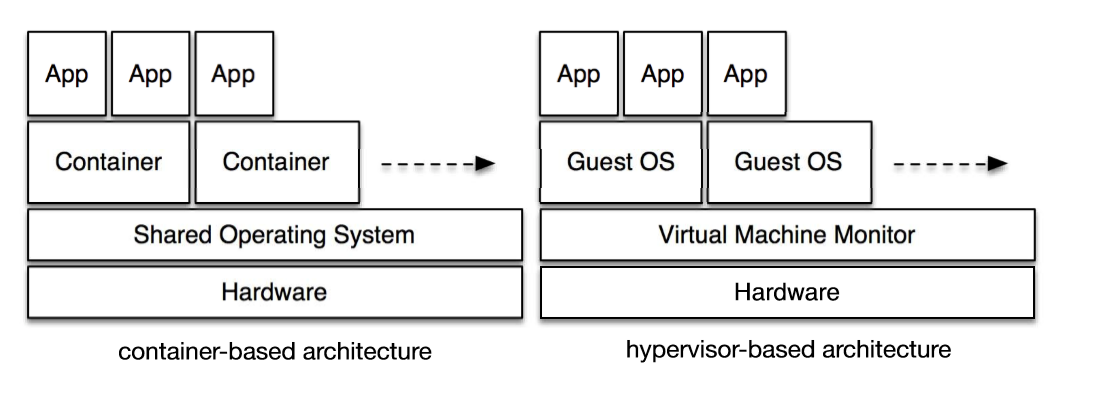
\includegraphics[width=1\linewidth]{pics/docker2.png}
	\captionof{figure}[Architektur]{Aufbau Container und Virtuelle Maschine \cite{Xavier2015AClouds}}
	\label{fig:architecture}
\end{minipage}

\subsubsection{Namespaces}
Dank der Einführung von Kernel Namespaces ist es möglich, Ressourcen des Host-Systems wie CPU, Arbeitsspeicher, I/O und Netzwerk voneinander zu isolieren und diese unter bestimmten Voraussetzungen anderen Anwendungen/Prozessen zur Verfügung zu stellen. 

Durch Namespaces werden die Ressourcen des Host System in Verschiedene Instanzen gepackt. Der innerhalb eines Namespaces gestartete Prozessaufruf sieht nur seine Eigene Instanz und die unterliegende Baumstruktur seiner Kind Prozesse. Der Prozess selbst hat die Illusion der Vollständigen Ressourcen Kontrolle über das komplette System, wobei Ihm nur ein zugewiesener Teil zur Verfügung steht.

Aktuell existieren sieben verschiedene Namespaces, Prozess ID (PID)-Namespaces, Mount-Namespaces, UTS-Namespaces, Interprocess Communication (IPC)-Namespaces, Network-Namespaces, User-Namespaces und Cgroup-Namespaces. Die im Folgenden genauer erklärt werden.

Die vereinfachte Darstellung des PID Namespaces einer gespawnten bzw geforkten Container-Prozess-Umgebung ist in Abbildung \ref{fig:PID} dargestellt. \cite{Liebel2017SkalierbareContainer-Infrastrukturen}

\vspace{1em}
\begin{minipage}{\linewidth}
	\centering
	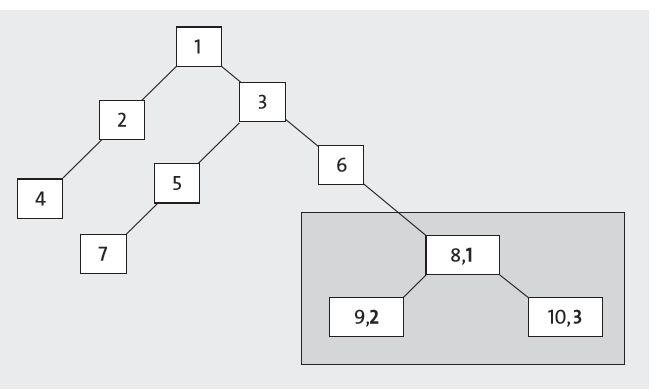
\includegraphics[width=1\linewidth]{pics/PID.PNG}
	\captionof{figure}[PID]{ PID Namespaces für Host und Container (im Fettdruck) \cite{Liebel2017SkalierbareContainer-Infrastrukturen}}
	\label{fig:PID}
\end{minipage}

\subparagraph{PID-Namespaces} sind hierarchisch deshalb kann ein Prozess nur die anderen Prozesse in seinem eigenen Namensraum oder in seinen untergeordneten Namensräumen sehen. Folglich kann der Host die Prozesse innerhalb des neuen PID-namespace des Containers beobachten und beeinflussen, aber die Prozesse innerhalb des Containers können die anderen Prozesse, die im Host oder in anderen Containern laufen, nicht beobachten oder beeinflussen

\subparagraph{Mount-Namespaces} isoliert filesystem Mountpunkte, die von einem Container gesehen werden, so dass Prozesse in verschiedenen Containern unterschiedliche Ansichten der File Systemhierarchie haben können.

\subparagraph{UTS-Namespaces} erlaubt es jedem Container seinen eigenen Hostnamen und NIS-Domänennamen zu haben.

\subparagraph{IPC-Namespaces} isoliert die Interprozesskommunikation, das bedeutet Prozesse, die in einem Container enthalten sind, haben eigene Nachrichten Warteschlangen und sind völlig unabhängig von Prozessen in anderen Containern.

\subparagraph{Network-Namespaces} isoliert das Netzwerk-Untersystem wie z.B. Geräte und IP-Adressen. Jeder Container unterhält seine eigene Netzwerk Konfiguration und die darauf laufenden Anwendungen.

\subparagraph{User-Namespaces} isoliert Benutzer-IDs vom Host und anderen laufenden Containern. Das bedeutet, dass der Benutzer Root (ID0) innerhalb eines Containers volle Privilegien hat, aber keine Privilegien außerhalb, was Sicherheit und Zuverlässigkeit gewährleistet. \cite{Xavier2015AClouds}

\subparagraph{Cgroup-Namespaces}
Isoliert Cgroup untereinander, dass keine Informationen über vorhandene Systemressourcen geteilt werden können.



\subsubsection{Cgroup}
\glqq Cgroup\grqq{} steht für \glqq Control group\grqq{}. Durch Cgroup ist es möglich, eine Reihe von Kriterien anzuwenden, um Ressourcen wie Speicher, Netzwerk, Festplatten-I/O und CPU einzuschränken. Ein Container sollte seine auferlegten Beschränkungen nicht überschreiten und andere Container, die auf derselben Hardware laufen, nicht stören. Cgroup ist für die Ressourcen Begrenzung, Priorisierung, Abrechnung und Kontrolle zuständig.

Durch Cgroup gibt es ein Weg, um Prozesse und System Ressourcen in einer kontrollierten und konfigurierbaren weise hierarchisch zu organisieren. Cgroup besteht im Wesentlichen aus zwei Teilen, dem Kern und dem Controller. Der Cgroup Kern ist in erster Linie für die hierarchische Organisation von Prozessen zuständig. Der Cgroup Controller ist in der Regel für die Verteilung einer bestimmten Art von System Ressource entlang der Hierarchie verantwortlich. Cgroup bilden eine Baumstruktur und jeder Prozess im System gehört genau zu einer Cgroup. Alle Unterprozesse (Kind Prozesse) eines Prozesses (Eltern Prozess) gehören zur gleichen cgroup.\cite{Heo2015ControlV2} 


\paragraph{Ressourcen Verteilungs Modelle}
Cgroup Controller verfügen über verschiedene Ressourcen Verteilungs Modelle. Die Modelle sind auf die Art und den Verwendungszweck der Ressource zugeschnitten. Dieser Paragraph befasst sich mit den verschiedenen Hauptschemen und deren Aufgaben \cite{Heo2015ControlV2}.

\subparagraph{Weight}
Beim Weight(Gewichtung) Modell werden die zur Verfügung stehenden Ressourcen eines Prozesses proportional zur Gewichtung an alle aktiven Kind Prozesse verteilt. Da nur die aktiven Kind Prozesse welche aktuell Ressourcen benötigen an der Verteilung teilnehmen, sind die zugeteilten Ressourcen effizient genutzt. 

\subparagraph{Limit}
Das Limit Modell bietet die Möglichkeit verschieden Limits zu verwenden. Ist ein High-Limit gesetzt, kann ein Kind Prozess die Ressource nur bis zu der konfigurierten Menge Verwenden. Low/High Limits können auch als soft-Limits bezeichnet werden. Die Summe der Limits aller Kind Prozesse kann die zur Verfügung stehende Menge an Ressourcen des Eltern Prozesses überschreiten. Ein Limit ist sozusagen ein maximaler Richtwert der bei dringendem Bedarf überschritten werden kann. Der Prozess welcher den über das Limit hinausragende Anteil verwendet, steht unter erhöhtem Druck und wird gedrängt die Ressource schnell wieder frei zu geben. Wenn eine Cgroup die Ressourcen nicht mehr benötigt, wird diese bis zu einem setzbaren Low-Limit freigegeben.


\subparagraph{Protection}
Im Protection Modell ist eine Cgroup so geschützt, dass sie bis zur konfigurierten Menge der Ressource fest zugeordnet werden kann, wenn die Verwendung aller Prozesse unter der geschützten Ebene Liegt. Der Schutz kann garantiert oder effizient sein. Bei garantiertem Schutz wird die Ressource explizit für die Cgroup freigehalten und kann vollständig verwendet werden. Die Effizientere Variante bietet die Möglichkeit zugeteilte Ressourcen auf Anfrage für andere Prozesse frei zu stellen.


\subparagraph{Allocation}
Einer Cgroup wird eine bestimmte Menge einer Ressource fest zugeteilt und stellt somit ein Hard-Limit dar. Die Summe der Zuweisungen von Kind Prozessen dürfen die Menge der fest zugeteilten Ressource des Eltern Prozesses nicht überschreiten. Auch wenn die Ressource nicht ausgenutzt wird, bleibt diese der Cgroup erhalten. 


\paragraph{Ressourcen Modellierung}
Da nicht jede Hardwareressource auf die gleiche Art eingeschränkt werden kann, existieren Controller die anhand der gerade beschriebenen Modelle Ressourcen Verwalten. Im folgenden Paragraphen werden die Art der Ressource mit verwendetem Modell genauer betrachtet und die Möglichkeiten für Administratoren unterschiedliche Varianten der Limitierung aufgezeigt. Besonderes Augenmerk ist auf die Speicherverwaltung gelegt.

\subparagraph{Speicher}
Der Speicher Controller regelt die Verteilung des Speichers. Speicher ist zustandsabhängig und verwendet sowohl Limit als auch Protection Modelle. Aufgrund der Verflechtung zwischen Speicherbedarf und Speicherrückgabeforderung ist die Verwaltung sehr kompliziert.

Memory-low(Best-effort)
Der geforderte Mindestanteil wird gestellt. Unbenutzter Speicher kann bei Bedarf vom System verwendet werden.

Memory-High(Best-effort)
Dies ist der Hauptmechanismus zur Steuerung des Speicherverbrauchs einer Cgroup. Wenn die Nutzung einer Cgroup über die obere Grenze hinausgeht, werden die Prozesse der Cgroup gedrosselt und unter starken Reklamationsdruck gesetzt.

Memory-min(Hard-Limit)
Falls der Speicherverbrauch einer Cgroup innerhalb seiner effektiven minimalen Grenze liegt, wird der Speicher der Cgroup unter keinen Umständen zurückgefordert. Wenn nicht genug Speicherplatz zur Verfügung steht um die Minimalanforderung zu gewährleisten, kommt der OOM-Killer (Später genauer beschrieben) zum Einsatz und schafft freien Speicher.

Memory-max(Hard-Limit)
Wenn der Speicherverbrauch einer Cgroup diese gesetzte Grenze erreicht und nicht reduziert werden kann, wird der OOM-Killer in der Cgroup aufgerufen, dies ist der letzte Schutzmechanismus. Unter bestimmten Umständen kann ein Prozess vorübergehend über das Limit hinaus gehen.

\subparagraph{CPU}
Der CPU Controller reguliert die Verteilung der CPU-Zyklen. Diese Steuerung Verwendet Gewichtung und Limit Modelle für normale Ressourcen Verteilung und das Allokation Modell für eine Echtzeit Verteilung.
\subparagraph{IO}
Der IO Controller reguliert die Verteilung der IO Ressourcen. Der Controller verwendet Gewichtung und Limit Modelle. Die Gewichtung gibt die relative IO-Zeit an, welche die Cgroup in Bezug auf ihre Geschwister verwenden kann.

\pagebreak
\subsection{Hypervisor-basierte Virtualisierung}
Eine Virtuelle Maschine Bildet mit Hilfe des \glqq{}\emph{Virtual Machine Monitor}\grqq{} (VMM) auch Hypervisor genannt eine komplette Rechnerarchitektur auf dem Host-Rechner nach (siehe Abbildung \ref{fig:architecture}). Der Hypervisor ist ein modifizierter minimaler Betriebssystem-Kernel. Man unterscheidet zwischen zwei Arten von VMM: Dem Typ 1 VMM oder \glqq{}\emph{Bare-Metal-Hypervisor}\grqq{}, welcher direkt auf der zugrundeliegenden Hardware des Hosts liegt und dem Typ-2-VMM \glqq{}\emph{hostet Hypervisor}\grqq{}, der eine komplette virtuelle Maschine auf dem Host Betriebssystem erstellt. Die Grundanforderung eines VMM sind nach Popek/Goldberg \cite{Popek1974FormalArchitectures,Glatz2015Betriebssysteme}:


 \subparagraph{Equivalence} 
 Prozesse welche auf der Virtuellen Maschine gestartet wurden, laufen mit Ausnahme der Geschwindigkeit identisch ab, wie Prozesse auf einem originalen Host-System.
 
\subparagraph{Efficiency} 
Alle unkritischen Prozesse werden von der Hardware direkt ausgeführt ohne eingreifen des VMM.

\subparagraph{Resource control} 
Es darf kein Prozess Ressourcen verwalten. Bei jedem zugriffsversuch eines Prozesses auf Systemressourcen wird der VMM aufgerufen.



\subsubsection{Typ-1-VMM}
Der Bare-Metal-Hypervisor in Abbildung \ref{fig:Hypervisor_Typ1/Typ2} a), Liegt direkt auf der Hardware und hat uneingeschränkten Zugriff darauf. Der VMM kümmert sich um die Ressourcenverwaltung und die Isolierte Bereitstellung von Virtuellen Maschinen. Die Aufteilung der Rechenzeit (CPU) und die Zuteilung von Speicher auf die einzelnen VMs sind Beispiele der Aufgaben welche die Ressourcenverwaltung beinhaltet. Xen \cite{Install2018XenArchitecture} und VMware ESX \cite{Go-to2018ESXi} verwendet diesen Virtualisierungs Ansatz, der nur mit einem eigenen auf die Hardware zugeschnittenen Treiber laufen kann \cite{Glatz2015Betriebssysteme}.

\vspace{1em}
\begin{minipage}{\linewidth}
	\centering
	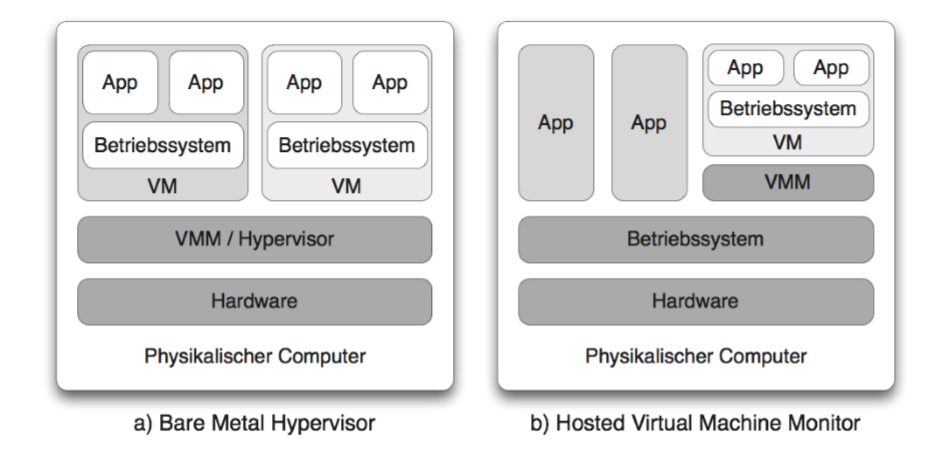
\includegraphics[width=1\linewidth]{pics/Hypervisoren.PNG}
	\captionof{figure}[Hypervisor Typ1/Type2]{Hypervisor Typ1/Typ2 \cite{Meinel2011VirtualisierungMarktubersicht} }
	\label{fig:Hypervisor_Typ1/Typ2}
\end{minipage}

\subsubsection{Typ-2-VMM}
Ein gehosteter-Hypervisor teilt sich ein Gastgeberbetriebssystem(Host-Betriebssystem) mit anderen Applikationen (siehe Abbildung \ref{fig:Hypervisor_Typ1/Typ2} b). Um die nötigen Rechte auf der Hardware zu erhalten, wird ein spezieller VMM-Treiber verwendet, der direkt unter dem Host-system installiert wird. Dieser ermöglicht Privilegierten Zugriff auf die Hardware. VMware Workstation und Virtual-Box sind Produkte dieser Realisierung der Virtualisierung \cite{Glatz2015Betriebssysteme}.

\subsubsection{Hybridformen}
Hypervisoren die von Haus aus direkt in das Betriebssystem integriert wurden, sind zwischen Typ 1 und Typ 2 anzusiedeln. Die Realisierung von Linux heißt KVM (Kernel-based Virtual Mashine), die Entwicklung von Windows ist Hyper-V. Diese Hybridformen sind die aktuell Performantesten Hypervisoren. 

\subsubsection{Hypervisor Virtualisierungsformen}
Egal, welche Methode der Virtualisierung zum Einsatz kommt, eins haben sie gemeinsam: Ressourcenanfragen die das Gastsystem an die CPU sendet, müssen von der Virtualisierungs Schicht (Hypervisor) abgefangen und interpretiert werden \cite{Meinel2011VirtualisierungMarktubersicht}. Das geschieht entweder über Vollständige-, Para- oder Hardwareunterstütze-Virtualisierung.  Es gibt bei aktuellen Prozessoren eine Rechteverwaltung welche man als Ringdiagramm darstellen kann (siehe Abbildung \ref{fig:Ringmodell1}). Im Ring 0 Besitzt man Volle Zugriffsrechte auf Hardware Ressourcen, auf dieser Ebene ist der Kernel beheimatet. Die Ringe 1 und 2 stehen für Treiber zur Verfügung und im Ring 3 wo die geringsten Zugriffsrechte enthalten sind, stehen alle sonstigen Anwendungen. Die Kernel der Gastbetriebssysteme befinden sich grundsätzlich ebenfalls in dem 3. Ring. Eine Zusammenstellung der Virtualisierungs Methoden ist in Abbildung \ref{fig:Virtualisierungen_Hypervisor} dargestellt.

\subparagraph{Vollständige-Virtualisierung}
 Wenn eine Anwendung mit einem Systemcall direkt auf einen vom Host-Kernel reservierten Speicherbereich zugreifen will, tritt eine Speicherschutzverletzung auf und der Zugriff wird verweigert, was den Prozess abstürzen lässt. Der Hypervisor fängt solche kritischen Anfragen ab, überprüft diese, Codiert die Anfragenstellung gegebenenfalls um und führt sie selbst mit Höheren Zugriffsrechten aus. Nach dem Aufruf folgt eine entsprechende Rückübersetzung und Rückgabe an die aufrufende virtuelle Maschine. Dieser Vorgang nennt man \glqq\emph{binary translation}\grqq{} und muss sehr häufig durchgeführt werden, was zu einem erheblichen Overhead führt, der signifikante Leistungseinbußen zur Folge hat \cite{Meinel2011VirtualisierungMarktubersicht}. 
 
 \vspace{1em}
\begin{minipage}{\linewidth}
	\centering
	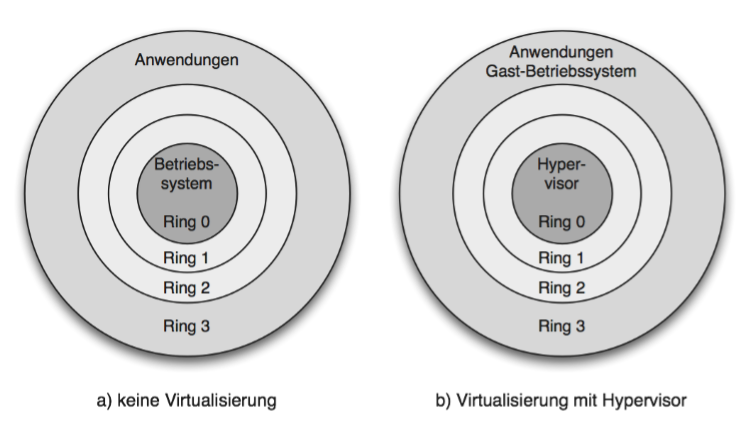
\includegraphics[width=1\linewidth]{pics/Ringmodell1.PNG}
	\captionof{figure}[Ringmodell 1 ]{Zugriffsrechteverwaltung mit und ohne Hypervisor \cite{Meinel2011VirtualisierungMarktubersicht} }
	\label{fig:Ringmodell1}
\end{minipage}
 
 \subparagraph{Para-Virtualisierung}
 Bei der Para-Virtualisierung werden die Kernel der Gastbetriebssysteme so angepasst, dass diese auf Ring 1 laufen können. Was vorher \emph{Systemcalls} waren und vom Betriebssystem verweigert wurden, sind jetzt \emph{Hypercalls} die direkt an den Hypervisor gesendet werden. Der Hypervisor führt den entsprechenden Systemaufruf aus und bedient die aufrufende virtuelle Maschine \cite{Meinel2011VirtualisierungMarktubersicht}. Um diese Effizientere Methode der Virtualisierung zu verwenden, ist darauf zugeschnittene Hardware nötig.

\vspace{1em}
\begin{minipage}{\linewidth}
	\centering
	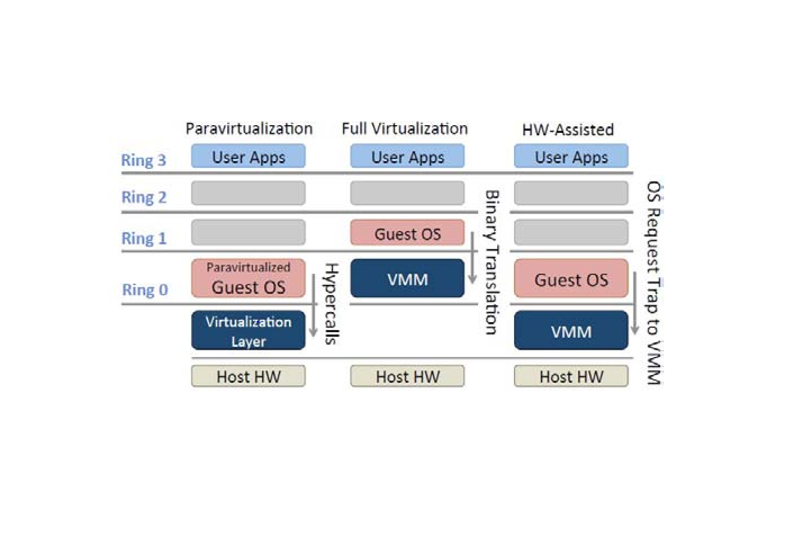
\includegraphics[width=1\linewidth]{pics/02Virtualisierungen_Hypervisor.PNG}
	\captionof{figure}[Virtualisierungen Hypervisor]{Virtualisierungen Hypervisor \cite{Fayyad-Kazan2013BenchmarkingHypervisors}}
	\label{fig:Virtualisierungen_Hypervisor}
\end{minipage}
 
\subparagraph{Hardwareunterstützte-Virtualisierun}
Durch die Hardware Unterstützung von Intel VT-x\cite{TechnologyIntel} oder AMD-v\cite{AMDVirtualisierungstechnologie} die den Prozessor-Befehlssatz erweitern, können virtuelle Maschinen System Calls nativ ausführen ohne die Kerne der Gastbetriebssysteme zu modifizieren, wie es bei der Para-Virtualisierung gemacht wird. Die Hardwareunterstützte Variante ist die Performanteste Methode der Hypervisor Technologien \cite{Meinel2011VirtualisierungMarktubersicht}.




%\pagebreak
